\documentclass[titlepage]{article}
\usepackage[T1]{fontenc}
\usepackage[utf8]{inputenc}
\usepackage{biblatex}
\usepackage{titling, lipsum}
\usepackage{graphicx}
\usepackage{indentfirst}
\usepackage{geometry}
\usepackage{hyperref} 
\usepackage{float}

\graphicspath{{./images/}}

\geometry{
 a4paper,
 total={170mm,257mm},
 margin=1in
}

\addbibresource{bibliography.bib}

\begin{document}
\begin{titlepage}
	{\centering
	{\scshape\huge Comparison of SLAM methods with CUDA implementation \par}
	\vspace{1cm}
	{\scshape\Large Course: Research project - GPU algorithms \par}}
	
	\vspace{1cm}
	\noindent\textbf{Coordinator}: Kaczmarski Krzysztof\\
	\textbf{Authors}: Rogala Michał, Stasiak Szymon, Śliwakowski Mateusz\\
	\textbf{Description}: This document covers three different SLAM methods with an emphasis on CUDA \mbox{implementation}\\
	\textbf{Code repository}: \href{https://github.com/Sliwson/cuda-slam}{https://github.com/Sliwson/cuda-slam}\\
	\textbf{Code license}: MIT\\
	\textbf{Input files}: Point clouds as .obj files\\

	\vfill
	{\large \today \par}
\end{titlepage}

\tableofcontents
\newpage

\section{Report goals}
%What we will know after reading this document?

The report is devoted to a research of SLAM methods using CUDA technology. We want to give a brief introduction what SLAM is and what are its applications. After reading the document you should know three different methods of approaching the problem, their advantages and disadvantages. The cornerstone of the work is answering the question - how well these methods can be converted to GPU architecture and how much will we gain?

\section{Problem statement}
%Description of the problem, motivating example, killer application, etc.

\subsection{Theoretical background}
\textbf{Simultaneous localization and mapping} (in short SLAM) is the computational problem of constructing or updating a map of an unknown environment while simultaneously keeping track of an agent's location within it \cite{ms-wiki1}. In theory the problem can be simplified to more mathematical definition - given two point sets $P_1 = \{x_1,\dots, x_n\}$ and $P_2=\{y_1, \dots, y_n\}$ find translation $t$ and rotation $R$ that minimizes the mean square error:
$$MSE(R, t) = \frac{1}{N}\sum_{i=1}{N}(x_i - Ry_i - t)^2$$

The reality, unfortunately, is much more complicated. Sizes of point sets might differ, clouds are unordered and noise points can occur.

\subsection{Applications}
The main field of SLAM application is robotics. There are a lot of machines that utilizes this algorithm to keep track of the space in which they are moving. The most popular are autonomous vacuum cleaners such as presented below.

\begin{figure}[H]
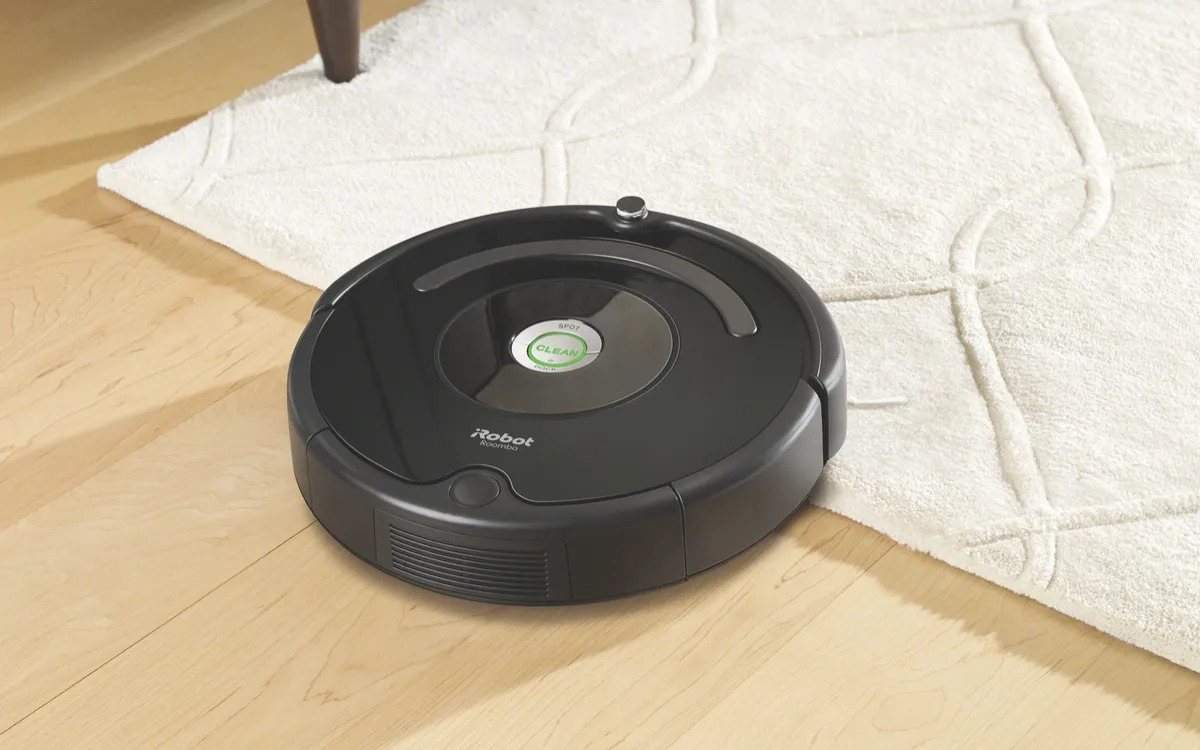
\includegraphics[width=\textwidth]{ms-img1.png}
\caption{Autonomous vacuum cleaner}
\end{figure}

Another popular application is mapping real life environments to digital equivalents. The programs produce \textit{Geospatial mappings} which can be later processed and analysed. Variety of different devices is used such as hand scanners, drone scanners or even satellites. Due to rapid technological progress nowadays, even smartphone cameras can be used to perform simple environmental scan.

\begin{figure}[H]
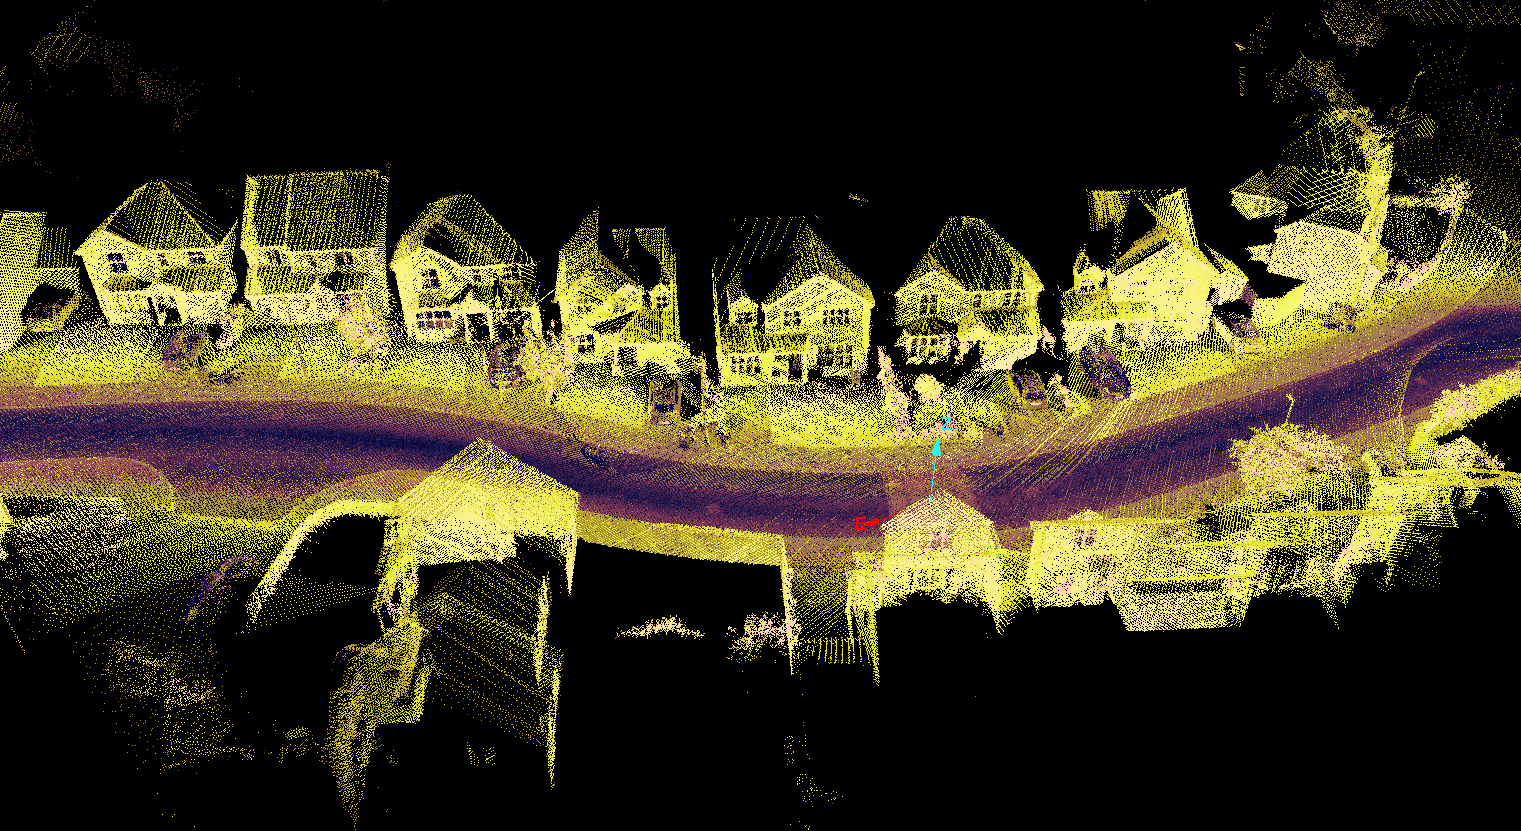
\includegraphics[width=\textwidth]{ms-img2.jpg}
\caption{3D laser scan}
\end{figure}

\section{Computational method}
%The most important ideas in the algorithm necessary to understand how it works.
%Are there any differences from other methods?
%Are there any novel ideas?

\subsection{Iterative Closest Point}
The most widely described and most popular method for solving SLAM problem is Iterative Closest Point algorithm. The main idea of the algorithm is stated below \cite{ms-pres1}:
\begin{enumerate}
\item Determine corresponding points.
\item Calculate translation and rotation using Singular Value Decomposition.
\item Apply calculated rotation and translation to the point cloud.
\item Compute Mean Squared Error.
\item If error decreased and it is greater than given threshold repeat all the steps.
\end{enumerate}

Various modifications have been proposed to this algorithm (such as sampling point sets, weighting the correspondences or rejecting outliers). However, in this project we focused on the base version of the method as it is good enough for comparison with the other algorithms.

\subsection{Noniterative Closest Point}
Interesting alternative to an iterative point cloud matching algorithms is a noniterative SVD-based solution. The idea have been described by Shinji Oomori, Takeshi Nishida, and Shuichi Kurogi of Kyushu Institute of Technology. Method is announced to match clouds "with less than 4\% of the computational
time of the ICP (iterative closest point) algorithm with nearly identical accuracy"\cite{nicp}.\\
The idea of algorithm is based on computing just two SVDs of large matrices built from respectively source and target points and multiplication of results. Unfortunately, for permuted clouds of different sizes this does not necesarilly mean the results always converge. In original solution this effect is reduced by running the computations for a few different perspectives of observed item. Therefore it can be used with promising results in situations where the item is observed from multiple angles.\\
Implementation described in this paper presents different approach - the clouds are randomly permuted and for the received result transformation, the mean squared error is computed for subcloud of given size.

\subsection{Coherent Point Drift}

\section{Program architecture}
%Short description on the modules of the system, requirements, dependencies, etc.
\subsection{Project structure}
The solution consists of three projects:
\begin{itemize}
\item \textit{common} - static library project, contains all elements that are shared between cpu and gpu implementations.
\item \textit{cpu-slam} - executable project, contains implementation of slam methods for cpu and cpu main.
\item \textit{gpu-slam} - executable project, contains implementaion of slam methods for gpu and gpu main.
\end{itemize}

\subsection{Modules}
The project is constructed using several modules:
\begin{itemize}
\item \textit{Renderer} - implemented in \textit{common} project. Capable of rendering point clouds in different colors. Can be used multiple times in one executable launch. Widely using for results visualisation.
\item \textit{CloudLoader} - implemented in \textit{common} project. Module responsible for loading .obj point clouds.
\item \textit{Configuration} - implemented in \textit{common} project. Module representing configuration, tightly coupled with \textit{ConfigParser} which allows loading configuration from .json files.
\item \textit{TestRunner} - implemented in \textit{common} project. Module used to define and run benchmarks.
\item \textit{Algorithms} - implemented in \textit{cuda-slam} as well as \textit{cpu-slam}. Each algorithm is implemented in separate file as a global function in appropriate namespace. Some operations that are common for cpu as well as gpu are implemented in \textit{common} project.
\end{itemize}

\subsection{Dependencies}
\begin{itemize}
\item \textit{Assimp} - for cloud loading.
\item \textit{Eigen} - for cpu matrix operations.
\item \textit{Glad} - wrapper for OpenGL.
\item \textit{GLFW} - for window system.
\item \textit{Nlohmann/json} - for configuration parsing.
\item \textit{cuBLAS}, \textit{cuSOLVER} - for gpu matrix operations.
\item \textit{glm} - 
\end{itemize}

\section{Input data description}
%File formats, api used to read, dependencies, data sources, etc.
%Is there any institution providing the input data?
%References to public databases.

As we wanted to keep the input simple we decided to use .obj files as the point clouds. It is easy to find multiple different models in this format which allowed us to test the algorithms on multiple distinctive samples. Furthermore, one can edit .obj files using for example \textit{Blender} to add noise or even cut off part of the cloud. We found that method most convenient to simulate real life conditions as 3D scanners data has to be processed using methods that are beyond the scope of our work.

\begin{figure}[H]
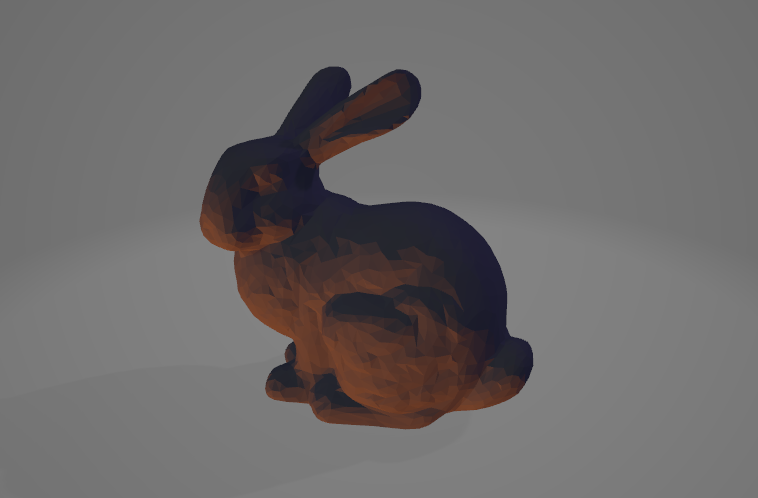
\includegraphics[width=\textwidth]{ms-bunny.png}
\caption{Sample .obj file}
\end{figure}

\section{Execution, configuration and user guide}
How can one replicate the experiments?
Any relevant information and runtime howtos.

\section{Implementation details}
%What do we thing is worth mentioning when it comes to implementation?
%What path has been chosen to parallelize execution especially for GPU?
%What obstacles have we met when implementing?
%Why have we chosen to use that libraries
\subsection{Common elements}
All of the methods implemented in scope of this project base to a greater or lesser extent on singular value decomposition (SVD) which has significant impact on quality of results and computation times. Unfortunately, there is no solid library offering that functionallity both for CPU and GPU computations. For this reason we decided to choose three libraries allowing us to receive satisfying results no matter what method is used:
\begin{itemize}
\item Eigen - widely recommended, open source library for CPU matrix operations
\item cuBLAS and cuSOLVER - library created and natively supported by Nvidia for GPU accelerated matrix operations
\item glm - OpenGL Mathematics library used mainly for storing common parts like point clouds, vectors, transformation matrices and basic operations on them. This library is avaliable also for device managed code what allows to reuse some parts of code for CPU and GPU managed computations and at the same time simplifies visualising the results
\end{itemize}
It is worth clarifying that Eigen has implemented the partial support for CUDA kernels but this feature is still experimental and there are multiple known issues (for example with support for gcc, MS Visual Studio). Adding that to potential problems with performance, we decided not to use this library for GPU accelerated operations in order to maintain higher scalability and stability of the project.

\subsection{Iterative Closest Point}

\subsection{Noniterative closest point}
The noniterative algorithm does not offer too many ways to take advantage from parallel CUDA operations. For that reason the most natural path for parallelizing the code is to parallely run SVDs for multiple permutations of source and target clouds. Unfortunately, natively supported solution from cuSOLVER library - batched SVD is not an option due to limitations for decomposed matrices size (it cannot be greater than 32 x 32 which corresponds point clouds of 32 points). For that reason another solution has been developed - each decomposition uses its own CUDA stream which are run parallely in batches of configured size.\\

\subsection{Coherent point drift}


\section{Description of the results}
%Performance of the system for different input data/parameters.
%How we understand the results and why are they correct?
%Can we formulate any conclusions from the experiments?

\subsection{Speed}

\subsection{Stability}

\subsection{Noise and outliers tolerance}

\subsection{Convergence ranges}

\section{Remarks}
Any remarks to the results and methods.

\section{Future works}
%What do we want to do in future, improvements.

\subsection{Iterative Closest Point}
We implemented a solid ground base for development of ICP algorithm. There are a lot of ways it can be improved but the most important would be enhancing performance of correspondences step as it is critical for the whole method execution time. 

\subsection{Noniterative Closest Point}
This method is for sure the poorest when it comes to documentation and papers dedicated to it. On the other hand, the idea does not leave much space for improvements. The biggest obstacle to using it on greater scale is undetermined convergence ratio. Although the tests conducted showed that running the alogrithm for 20 pseudo-random permutations gives convergence ratio of 100\% but the actual corellation between computation precision and cloud properties such as size or density remains unknown.\\
Other place for improvements is related closely to implementation issue. Different libraries and methods of computing SVD offers different accuracy. This can be seen for example by comparing results of CPU computations using Eigen library (recommended as one of the top when it comes to finding matrix decomposition) and GPU's cuSOLVER, where for the second one, error is smaller in majority of test cases. There are also multiple other, both closed and open source implementations for both CPU and GPU which might offer better results when it comes to convergence or computation time, especially for some specific cases.

\subsection{Common improvements}
The key to performant SLAM for big clouds is sampling. We haven't covered it in our work as it is a broad topic and mostly dependent of the specific application of the algorithm. Although, there is no contraindication to use sampled clouds as the input of our program so everybody can make their own experiments in that field.

\newpage
\printbibliography

\end{document}

